%%%% Paramétrage du TD %%%%
\def\xxactivite{TD 5 \ifprof -- Corrigé \else \fi} % \normalsize \vspace{-.4cm}
\def\xxauteur{\textsl{Xavier Pessoles}}


\def\xxnumchapitre{Chapitre 1 \vspace{.2cm}}
\def\xxchapitre{\hspace{.12cm} Correction des systèmes}


\def\xxcompetences{%
\vspace{-.3cm}
\textsl{%
\textbf{Savoirs et compétences :}\\
\vspace{-.4cm}
\begin{itemize}[label=\ding{112},font=\color{ocre}] 
%\item \textit{Res1.C4 : } Correction
\item \textit{Res1.C4.SF1 : } Proposer la démarche de réglage d’un correcteur proportionnel, 
proportionnel intégral 
%et à avance de phase
\item \textit{Con.C2 : } 	Correction d’un système asservi	
%\item \textit{Con.C2.SF1 : } Choisir un type de correcteur adapté
\end{itemize}
}}

\def\xxtitreexo{Banc d’épreuve hydraulique}
\def\xxsourceexo{\hspace{.2cm} CCP -- PSI -- 2010}
\def\xxauteur{\textsl{Xavier Pessoles}}

\def\xxfigures{
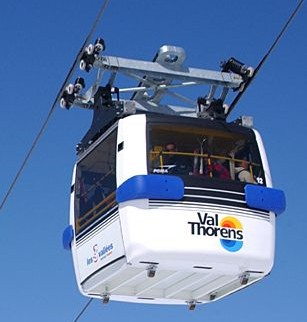
\includegraphics[width=.7\linewidth]{fig_00}
}%figues de la page de garde


\iflivret
\pagestyle{empty}


%%%%%%%% PAGE DE GARDE COURS
\ifcours
\begin{tikzpicture}[remember picture,overlay]
\node at (current page.north west)
{\begin{tikzpicture}[remember picture,overlay]
\node[anchor=north west,inner sep=0pt] at (0,0) {\includegraphics[width=\paperwidth]{\thechapterimage}};
\draw[anchor=west] (-2cm,-8cm) node [line width=2pt,rounded corners=15pt,draw=ocre,fill=white,fill opacity=0.6,inner sep=40pt]{\strut\makebox[22cm]{}};
\draw[anchor=west] (1cm,-8cm) node {\huge\sffamily\bfseries\color{black} %
\begin{minipage}{1cm}
\rotatebox{90}{\LARGE\sffamily\textsc{\color{ocre}\textbf{\xxnumpartie}}}
\end{minipage} \hfill
\begin{minipage}[c]{14cm}
\begin{titrepartie}
\begin{flushright}
\renewcommand{\baselinestretch}{1.1} 
\Large\sffamily\textsc{\textbf{\xxpartie}}
\renewcommand{\baselinestretch}{1} 
\end{flushright}
\end{titrepartie}
\end{minipage} \hfill
\begin{minipage}[c]{3.5cm}
{\large\sffamily\textsc{\textbf{\color{ocre} \discipline}}}
\end{minipage} 
 };
\end{tikzpicture}};
\end{tikzpicture}


\begin{tikzpicture}[overlay]
\node[shape=rectangle, 
      rounded corners = .25 cm,
	  draw= ocre,
	  line width=2pt, 
	  fill = ocre!10,
	  minimum width  = 2.5cm,
	  minimum height = 3cm,] at (18cm,0) {};
\node at (17.7cm,0) {\rotatebox{90}{\textbf{\Large\color{ocre}{\classe}}}};
%{};
\end{tikzpicture}

\vspace{3.5cm}

\begin{tikzpicture}[remember picture,overlay]
\draw[anchor=west] (-2cm,-6cm) node {\huge\sffamily\bfseries\color{black} %
\begin{minipage}{2cm}
\begin{center}
\LARGE\sffamily\textsc{\color{ocre}\textbf{\xxactivite}}
\end{center}
\end{minipage} \hfill
\begin{minipage}[c]{15cm}
\begin{titrechapitre}
\renewcommand{\baselinestretch}{1.1} 
\Large\sffamily\textsc{\textbf{\xxnumchapitre}}

\Large\sffamily\textsc{\textbf{\xxchapitre}}
\vspace{.5cm}

\renewcommand{\baselinestretch}{1} 
\normalsize\normalfont
\xxcompetences
\end{titrechapitre}
\end{minipage}  };
\end{tikzpicture}
\vfill

\begin{flushright}
\begin{minipage}[c]{.3\linewidth}
\begin{center}
\xxfigures
\end{center}
\end{minipage}\hfill
\begin{minipage}[c]{.6\linewidth}
\startcontents
\printcontents{}{1}{}
\end{minipage}
\end{flushright}

\begin{tikzpicture}[remember picture,overlay]
\draw[anchor=west] (4.5cm,-.7cm) node {
\begin{minipage}[c]{.2\linewidth}
\begin{flushright}

\includegraphics[width=2cm]{png/logoCC}
\end{flushright}
\end{minipage}
\begin{minipage}[c]{.2\linewidth}
\textsl{\xxauteur} \\
\textsl{\classe}
\end{minipage}
 };
\end{tikzpicture}
\newpage
\pagestyle{fancy}

\newpage
\pagestyle{fancy}

\else
\fi


%%%%%%%% PAGE DE GARDE TD
\iftd
%\begin{tikzpicture}[remember picture,overlay]
%\node at (current page.north west)
%{\begin{tikzpicture}[remember picture,overlay]
%\draw[anchor=west] (-2cm,-3.25cm) node [line width=2pt,rounded corners=15pt,draw=ocre,fill=white,fill opacity=0.6,inner sep=40pt]{\strut\makebox[22cm]{}};
%\draw[anchor=west] (1cm,-3.25cm) node {\huge\sffamily\bfseries\color{black} %
%\begin{minipage}{1cm}
%\rotatebox{90}{\LARGE\sffamily\textsc{\color{ocre}\textbf{\xxnumpartie}}}
%\end{minipage} \hfill
%\begin{minipage}[c]{13.5cm}
%\begin{titrepartie}
%\begin{flushright}
%\renewcommand{\baselinestretch}{1.1} 
%\Large\sffamily\textsc{\textbf{\xxpartie}}
%\renewcommand{\baselinestretch}{1} 
%\end{flushright}
%\end{titrepartie}
%\end{minipage} \hfill
%\begin{minipage}[c]{3.5cm}
%{\large\sffamily\textsc{\textbf{\color{ocre} \discipline}}}
%\end{minipage} 
% };
%\end{tikzpicture}};
%\end{tikzpicture}

%%%%%%%%%% PAGE DE GARDE TD %%%%%%%%%%%%%%%
%\begin{tikzpicture}[overlay]
%\node[shape=rectangle, 
%      rounded corners = .25 cm,
%	  draw= ocre,
%	  line width=2pt, 
%	  fill = ocre!10,
%	  minimum width  = 2.5cm,
%	  minimum height = 2.5cm,] at (18.5cm,0) {};
%\node at (17.7cm,0) {\rotatebox{90}{\textbf{\Large\color{ocre}{\classe}}}};
%%{};
%\end{tikzpicture}

% PARTIE ET CHAPITRE
%\begin{tikzpicture}[remember picture,overlay]
%\draw[anchor=west] (-1cm,-2.1cm) node {\large\sffamily\bfseries\color{black} %
%\begin{minipage}[c]{15cm}
%\begin{flushleft}
%\xxnumchapitre \\
%\xxchapitre
%\end{flushleft}
%\end{minipage}  };
%\end{tikzpicture}

% Bandeau titre exo
\begin{tikzpicture}[remember picture,overlay]
\draw[anchor=west] (-2cm,-6cm) node {\huge\sffamily\bfseries\color{black} %
\begin{minipage}{5cm}
\begin{center}
\LARGE\sffamily\color{ocre}\textbf{\textsc{\xxactivite}}

\begin{center}
\xxfigures
\end{center}

\end{center}
\end{minipage} \hfill
\begin{minipage}[c]{12cm}
\begin{titrechapitre}
\renewcommand{\baselinestretch}{1.1} 
\large\sffamily\textbf{\textsc{\xxtitreexo}}

\small\sffamily{\textbf{\textit{\color{black!70}\xxsourceexo}}}
\vspace{.5cm}

\renewcommand{\baselinestretch}{1} 
\normalsize\normalfont
\xxcompetences
\end{titrechapitre}
\end{minipage}  };
\end{tikzpicture}

\else
\fi


%%%%%%%% PAGE DE GARDE FICHE
\iffiche
\begin{tikzpicture}[remember picture,overlay]
\node at (current page.north west)
{\begin{tikzpicture}[remember picture,overlay]
\draw[anchor=west] (-2cm,-3.25cm) node [line width=2pt,rounded corners=15pt,draw=ocre,fill=white,fill opacity=0.6,inner sep=40pt]{\strut\makebox[22cm]{}};
\draw[anchor=west] (1cm,-3.25cm) node {\huge\sffamily\bfseries\color{black} %
\begin{minipage}{1cm}
\rotatebox{90}{\LARGE\sffamily\textsc{\color{ocre}\textbf{\xxnumpartie}}}
\end{minipage} \hfill
\begin{minipage}[c]{14cm}
\begin{titrepartie}
\begin{flushright}
\renewcommand{\baselinestretch}{1.1} 
\large\sffamily\textsc{\textbf{\xxpartie} \\} 

\vspace{.2cm}

\normalsize\sffamily\textsc{\textbf{\xxnumchapitre -- \xxchapitre}}
\renewcommand{\baselinestretch}{1} 
\end{flushright}
\end{titrepartie}
\end{minipage} \hfill
\begin{minipage}[c]{3.5cm}
{\large\sffamily\textsc{\textbf{\color{ocre} \discipline}}}
\end{minipage} 
 };
\end{tikzpicture}};
\end{tikzpicture}


\begin{tikzpicture}[overlay]
\node[shape=rectangle, 
      rounded corners = .25 cm,
	  draw= ocre,
	  line width=2pt, 
	  fill = ocre!10,
	  minimum width  = 2.5cm,
%	  minimum height = 2.5cm,] at (18.5cm,0.5cm) {};
	  minimum height = 2.5cm,] at (18.5cm,0cm) {};
\node at (17.7cm,0) {\rotatebox{90}{\textsf{\textbf{\large\color{ocre}{\classe}}}}};
%{};
\end{tikzpicture}



\else
\fi



\else
\pagestyle{empty}


%%%%%%%% PAGE DE GARDE COURS
\ifcours
\begin{tikzpicture}[remember picture,overlay]
\node at (current page.north west)
{\begin{tikzpicture}[remember picture,overlay]
\node[anchor=north west,inner sep=0pt] at (0,0) {\includegraphics[width=\paperwidth]{\thechapterimage}};
\draw[anchor=west] (-2cm,-8cm) node [line width=2pt,rounded corners=15pt,draw=ocre,fill=white,fill opacity=0.6,inner sep=40pt]{\strut\makebox[22cm]{}};
\draw[anchor=west] (1cm,-8cm) node {\huge\sffamily\bfseries\color{black} %
\begin{minipage}{1cm}
\rotatebox{90}{\LARGE\sffamily\textsc{\color{ocre}\textbf{\xxnumpartie}}}
\end{minipage} \hfill
\begin{minipage}[c]{14cm}
\begin{titrepartie}
\begin{flushright}
\renewcommand{\baselinestretch}{1.1} 
\Large\sffamily\textsc{\textbf{\xxpartie}}
\renewcommand{\baselinestretch}{1} 
\end{flushright}
\end{titrepartie}
\end{minipage} \hfill
\begin{minipage}[c]{3.5cm}
{\large\sffamily\textsc{\textbf{\color{ocre} \discipline}}}
\end{minipage} 
 };
\end{tikzpicture}};
\end{tikzpicture}


\begin{tikzpicture}[overlay]
\node[shape=rectangle, 
      rounded corners = .25 cm,
	  draw= ocre,
	  line width=2pt, 
	  fill = ocre!10,
	  minimum width  = 2.5cm,
	  minimum height = 3cm,] at (18cm,0) {};
\node at (17.7cm,0) {\rotatebox{90}{\textbf{\Large\color{ocre}{\classe}}}};
%{};
\end{tikzpicture}

\vspace{3.5cm}

\begin{tikzpicture}[remember picture,overlay]
\draw[anchor=west] (-2cm,-6cm) node {\huge\sffamily\bfseries\color{black} %
\begin{minipage}{2cm}
\begin{center}
\LARGE\sffamily\textsc{\color{ocre}\textbf{\xxactivite}}
\end{center}
\end{minipage} \hfill
\begin{minipage}[c]{15cm}
\begin{titrechapitre}
\renewcommand{\baselinestretch}{1.1} 
\Large\sffamily\textsc{\textbf{\xxnumchapitre}}

\Large\sffamily\textsc{\textbf{\xxchapitre}}
\vspace{.5cm}

\renewcommand{\baselinestretch}{1} 
\normalsize\normalfont
\xxcompetences
\end{titrechapitre}
\end{minipage}  };
\end{tikzpicture}
\vfill

\begin{flushright}
\begin{minipage}[c]{.3\linewidth}
\begin{center}
\xxfigures
\end{center}
\end{minipage}\hfill
\begin{minipage}[c]{.6\linewidth}
\startcontents
\printcontents{}{1}{}
\end{minipage}
\end{flushright}

\begin{tikzpicture}[remember picture,overlay]
\draw[anchor=west] (4.5cm,-.7cm) node {
\begin{minipage}[c]{.2\linewidth}
\begin{flushright}

\includegraphics[width=2cm]{png/logoCC}
\end{flushright}
\end{minipage}
\begin{minipage}[c]{.2\linewidth}
\textsl{\xxauteur} \\
\textsl{\classe}
\end{minipage}
 };
\end{tikzpicture}
\newpage
\pagestyle{fancy}

\newpage
\pagestyle{fancy}

\else
\fi


%%%%%%%% PAGE DE GARDE TD
\iftd
%\begin{tikzpicture}[remember picture,overlay]
%\node at (current page.north west)
%{\begin{tikzpicture}[remember picture,overlay]
%\draw[anchor=west] (-2cm,-3.25cm) node [line width=2pt,rounded corners=15pt,draw=ocre,fill=white,fill opacity=0.6,inner sep=40pt]{\strut\makebox[22cm]{}};
%\draw[anchor=west] (1cm,-3.25cm) node {\huge\sffamily\bfseries\color{black} %
%\begin{minipage}{1cm}
%\rotatebox{90}{\LARGE\sffamily\textsc{\color{ocre}\textbf{\xxnumpartie}}}
%\end{minipage} \hfill
%\begin{minipage}[c]{13.5cm}
%\begin{titrepartie}
%\begin{flushright}
%\renewcommand{\baselinestretch}{1.1} 
%\Large\sffamily\textsc{\textbf{\xxpartie}}
%\renewcommand{\baselinestretch}{1} 
%\end{flushright}
%\end{titrepartie}
%\end{minipage} \hfill
%\begin{minipage}[c]{3.5cm}
%{\large\sffamily\textsc{\textbf{\color{ocre} \discipline}}}
%\end{minipage} 
% };
%\end{tikzpicture}};
%\end{tikzpicture}

%%%%%%%%%% PAGE DE GARDE TD %%%%%%%%%%%%%%%
%\begin{tikzpicture}[overlay]
%\node[shape=rectangle, 
%      rounded corners = .25 cm,
%	  draw= ocre,
%	  line width=2pt, 
%	  fill = ocre!10,
%	  minimum width  = 2.5cm,
%	  minimum height = 2.5cm,] at (18.5cm,0) {};
%\node at (17.7cm,0) {\rotatebox{90}{\textbf{\Large\color{ocre}{\classe}}}};
%%{};
%\end{tikzpicture}

% PARTIE ET CHAPITRE
%\begin{tikzpicture}[remember picture,overlay]
%\draw[anchor=west] (-1cm,-2.1cm) node {\large\sffamily\bfseries\color{black} %
%\begin{minipage}[c]{15cm}
%\begin{flushleft}
%\xxnumchapitre \\
%\xxchapitre
%\end{flushleft}
%\end{minipage}  };
%\end{tikzpicture}

% Bandeau titre exo
\begin{tikzpicture}[remember picture,overlay]
\draw[anchor=west] (-2cm,-6cm) node {\huge\sffamily\bfseries\color{black} %
\begin{minipage}{5cm}
\begin{center}
\LARGE\sffamily\color{ocre}\textbf{\textsc{\xxactivite}}

\begin{center}
\xxfigures
\end{center}

\end{center}
\end{minipage} \hfill
\begin{minipage}[c]{12cm}
\begin{titrechapitre}
\renewcommand{\baselinestretch}{1.1} 
\large\sffamily\textbf{\textsc{\xxtitreexo}}

\small\sffamily{\textbf{\textit{\color{black!70}\xxsourceexo}}}
\vspace{.5cm}

\renewcommand{\baselinestretch}{1} 
\normalsize\normalfont
\xxcompetences
\end{titrechapitre}
\end{minipage}  };
\end{tikzpicture}

\else
\fi


%%%%%%%% PAGE DE GARDE FICHE
\iffiche
\begin{tikzpicture}[remember picture,overlay]
\node at (current page.north west)
{\begin{tikzpicture}[remember picture,overlay]
\draw[anchor=west] (-2cm,-3.25cm) node [line width=2pt,rounded corners=15pt,draw=ocre,fill=white,fill opacity=0.6,inner sep=40pt]{\strut\makebox[22cm]{}};
\draw[anchor=west] (1cm,-3.25cm) node {\huge\sffamily\bfseries\color{black} %
\begin{minipage}{1cm}
\rotatebox{90}{\LARGE\sffamily\textsc{\color{ocre}\textbf{\xxnumpartie}}}
\end{minipage} \hfill
\begin{minipage}[c]{14cm}
\begin{titrepartie}
\begin{flushright}
\renewcommand{\baselinestretch}{1.1} 
\large\sffamily\textsc{\textbf{\xxpartie} \\} 

\vspace{.2cm}

\normalsize\sffamily\textsc{\textbf{\xxnumchapitre -- \xxchapitre}}
\renewcommand{\baselinestretch}{1} 
\end{flushright}
\end{titrepartie}
\end{minipage} \hfill
\begin{minipage}[c]{3.5cm}
{\large\sffamily\textsc{\textbf{\color{ocre} \discipline}}}
\end{minipage} 
 };
\end{tikzpicture}};
\end{tikzpicture}


\begin{tikzpicture}[overlay]
\node[shape=rectangle, 
      rounded corners = .25 cm,
	  draw= ocre,
	  line width=2pt, 
	  fill = ocre!10,
	  minimum width  = 2.5cm,
%	  minimum height = 2.5cm,] at (18.5cm,0.5cm) {};
	  minimum height = 2.5cm,] at (18.5cm,0cm) {};
\node at (17.7cm,0) {\rotatebox{90}{\textsf{\textbf{\large\color{ocre}{\classe}}}}};
%{};
\end{tikzpicture}



\else
\fi



\fi
\setlength{\columnseprule}{.1pt}

\pagestyle{fancy}
\thispagestyle{plain}

\vspace{4.9cm}

\def\columnseprulecolor{\color{ocre}}
\setlength{\columnseprule}{0.4pt} 

%%%%%%%%%%%%%%%%%%%%%%%


\begin{multicols}{2}
\setcounter{exo}{0}

%\section{Banc d'épreuve hydraulique}
\subsection*{Présentation}
\ifprof
\else
Vallourec \& Mannesmann Tubes (V\&M Tubes), entreprise du groupe Vallourec, est le leader mondial dans la production de tubes en acier sans soudure laminés à chaud. %L’entreprise exploite des tuberies équipées des installations les plus modernes : quatre en France, quatre en Allemagne, trois  aux USA et au Brésil et une ligne de finition en Chine.
%Les tubes sans soudure en acier produits par V\&M Tubes couvrent une très large gamme tant sur le plan dimensionnel que dans la nature des matériaux.
% :
%•	les diamètres extérieurs vont de 21,3 mm à 1,5 m, les épaisseurs de 2 à 250 mm ;
%•	outre les aciers non alliés et alliés, V&M Tubes produit des tubes en aciers spéciaux élaborés pour s’adapter aux applications spécifiques des clients.
%Ces tubes sont employés dans des applications très diverses : 
%•	canalisations hydrauliques, pneumatiques, vapeur ;
%•	ventilation, climatisation ;
%•	en basse pression ou haute pression…
%Les industries utilisatrices sont tout aussi variées. Pour certaines d’entre elles, telles que les industries pétrolières ou nucléaires par exemple, où les problèmes de sécurité sont particulièrement importants, il arrive que les clients exigent des qualités spécifiques pour leurs tubes en plus des critères liés au cahier des charges standard. Une de ces contraintes personnalisées est la garantie de la tenue des tubes à un seuil de pression durant un temps donné.
%Le site de V\&M Tubes situé à Aulnoye-Aymeries, qui produit des tubes de 114 mm à 508 mm de diamètre pour des longueurs variant de 4,40 à 14,20 m possède un banc spécifique de test de pression hydraulique pour valider la qualité des produits finis exigée par certains clients. C’est le fonctionnement de ce banc conçu par M\&T Tubes qui fait l’objet de cette étude.

Afin de valider la caractéristique de tenue en pression des tubes, ceux-ci sont soumis à une pression hydraulique donnée durant un temps spécifié. Ces paramètres dépendent de la taille des tubes et de leur future utilisation.

%\subsection{Analyse de la fonction technique << mettre le tube sous pression >>.}
%
%La finalité de la mise sous pression est de vérifier la résistance du tube pour une pression maximale imposée par le client. Le cahier des charges impose un écart statique en pression inférieur à 5\% et aucun dépassement. 
%Les objectifs de cette partie sont de modéliser le système de mise sous pression afin de vérifier le respect de ce cahier des charges et au besoin de proposer des modifications de la commande pour pallier les écarts observés.
%
Un schéma hydraulique simplifié est donné figure suivante :
\begin{center}
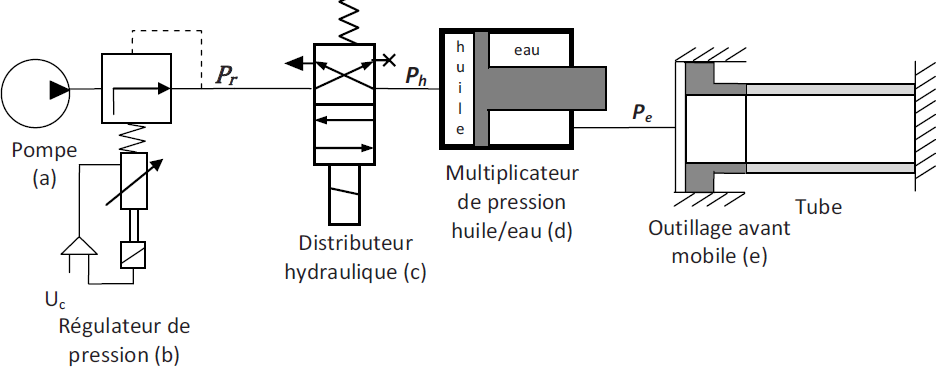
\includegraphics[width=\linewidth]{fig_01}
\end{center}
%
%
%\begin{itemize}
%\item Le fluide injecté dans le tube est de l’eau sous pression.
%\item Dans un premier temps, l’opérateur règle la tension consigne Uc de mise sous pression par l’intermédiaire d’un potentiomètre (non représenté), une plage de tension de 0 à \SI{2,5}{V} correspondant à une consigne de pression d’eau comprise entre 0 et \SI{1000}{bars}.
%\item La pompe (a) fournit de l’huile dont la pression est réglée par un régulateur de pression (b) piloté par cette tension consigne $U_c$.
%\item Un distributeur hydraulique (c) pilote la montée d’un multiplicateur de pression huile/eau (d) ;
%Ph désigne la pression d’huile en entrée et $P_e$ la  pression d’eau en sortie.
%\item L’eau est injectée par l’outillage avant (e) dans le tube. Sa pression est mesurée par un capteur de pression de gain $K_{cap} = 2,5\cdot 10^{-3} \text{V/bars}$  (non représenté).
%\end{itemize}
%
%\subsubsection{Mise en place du modèle}
%
%Jusqu’à la Question 24, on négligera le temps de réponse de cet ensemble face à la dynamique du distributeur, du multiplicateur de pression et de l’outillage avant de mise sous pression. On supposera donc que la pression en sortie du régulateur est constante, égale à $P_r$.
%
%Le distributeur hydraulique fournit un débit d’huile défini par l’équation : 
%	$Q_h (t)=K_r.\sqrt{P_r (t)-P_h (t)}$, avec $K_r$ constante en $\text{m}^3.\text{Pa}^{-1/2}$, avec :
%\begin{itemize}
%\item $P_r(t)$ : pression en entrée du distributeur (sortie du régulateur);
%\item $P_h(t)$ : pression en sortie du distributeur.
%\end{itemize}
%
%
%\begin{minipage}[c]{.65\linewidth}
%Le multiplicateur, représenté ci-contre, se compose d’un piston, de masse $M$, en translation par rapport au bâti, séparant les chambres $C_e$ et $C_h$ comportant respectivement de l’eau et de l’huile sous pression.
%On note :
%\begin{itemize}
%\item $Q_e(t)$ : le débit volumique d’eau en sortie du multiplicateur;
%\item $Q_h(t)$ : le débit volumique d’huile en entrée du multiplicateur;
%\item $P_e(t)$ : la pression d’eau dans $C_e$;
%\item $P_h(t)$ : la pression d’huile dans $C_h$;
%\item $z(t)$ : la position du piston;
%\item $V_e(t)$ : le volume de $C_e$;
%\item $V_h(t)$ : le volume de $C_h$;
%\item $g$ : l’accélération de pesanteur;
%\item $\vect{z}$ : le vecteur vertical unitaire ascendant.
%\end{itemize}
%
%Les équations du débit sont : 
%$$
%	Q_e (t)=S_e\dfrac{\text{d}z(t)}{\text{d}t}-\dfrac{V_{e0}}{B_e}   \dfrac{\text{d}P_e (t)}{\text{d}t}
%\quad
%	Q_h (t)=S_h\dfrac{\text{d}z(t)}{\text{d}t}+\dfrac{V_{h0}}{B_h}   \dfrac{\text{d}P_h (t)}{\text{d}t}
%$$
%\end{minipage}\hfill
%\begin{minipage}[c]{.3\linewidth}
%\begin{center}
%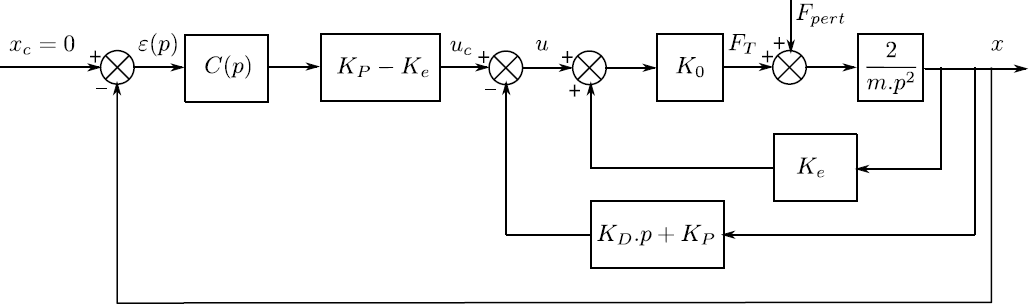
\includegraphics[width=\linewidth]{fig_02}
%%\textit{Schéma d'asservissement de la vitesse des vis $3_k$.}
%\end{center}
%\end{minipage}
%
%Données numériques : 
%\begin{multicols}{2}
%\begin{itemize}
%\item $S_e$ :	section du piston dans la chambre $C_e = \SI{397,6}{10^{-4}m^2}$;
%\item $S_h$ :	section du piston dans la chambre $C_h = \SI{1288,25}{10^{-4}m^2}$;
%\item $B_e$ :	module de compressibilité de l’eau = \SI{2.109}{Pa};
%\item $B_h$ :	module de compressibilité de l’huile = \SI{109}{Pa};
%\item $M$ :	masse du piston = \SI{668}{kg};
%\item $f$ :	coefficient de frottement visqueux = $10^6 \, \text{N/m/s}$;
%\item $V_{e0}$ :	volume initial de la chambre $C_e =  1,2.10^{-2}\,\text{m}^3$;
%\item $V_{h0}$ :	volume initial de la chambre $C_h = 3,8.10^{-2}\,\text{m}^3$.
%\end{itemize}
%\end{multicols}
%En appliquant le théorème de la résultante dynamique selon $\vect{z}$ sur le piston du multiplicateur, on a : 
%$$
%M\ddot{z}(t)=S_hp_h(t)-S_ep_e(t)-Mg-f\dot{z}(t).
%$$
%\subparagraph{}
%\textit{Déduire de la relation précédente l’équation reliant $Z(p)$, $P_e(p)$, $P_h(p)$, et $\text{Poids}(p)=Mg/p$, transformées de Laplace de $z(t)$, $P_e(t)$, $P_h(t)$ et du poids perçu comme une perturbation. Les conditions initiales sont supposées nulles.}
%
%\subsubsection{Modélisation du chariot avant}
%Le chariot avant comporte :
%\begin{itemize}
%\item la traverse, mise en position par un vérin hydraulique avant la mise sous pression du tube. Durant toute la durée de l’épreuve, on supposera que la traverse est immobile par rapport au bâti;
%\item un équipage mobile sur lequel est monté l’outillage, en translation rectiligne par rapport à la traverse.
%\end{itemize}
%
%
%
%\begin{center}
%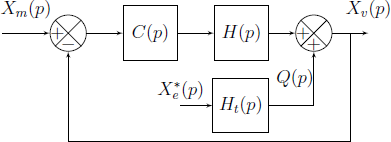
\includegraphics[width=.8\linewidth]{fig_03}
%%\textit{Schéma d'asservissement de la vitesse des vis $3_k$.}
%\end{center}
%
%
%On note :
%\begin{itemize}
%	\item $L(t)$ la position de l’équipage mobile repérée par rapport à sa position initiale;
%	\item $V_t(t)$ le volume du tube;
%	\item $F_t(t)$ l’effort du tube sur l’équipage mobile, avec $F_t(t) = - rL(t)$.
%\end{itemize}
%
%On néglige les variations de volume du tube dues à ses déformations. L’équation du débit s’écrit alors :
%	$$Q_e (t)=(S_a-S_b ).\dfrac{\text{d}L(t)}{\text{d}t}+\dfrac{V_t}{B_e}  \dfrac{\text{d}P_e (t)}{\text{d}t}.$$
%	
%	
%Données numériques :
%\begin{itemize}
%	\item $S_a$ et $S_b$ :	sections de l’équipage mobile côté tube et côté opposé au tube,
%$S_a -S_b  = \SI{1,88}{10^{-3}.m^2}$;	
%	\item $m$ :		masse de l’ensemble mobile = \SI{25}{kg};
%	\item $f ’$ :		coefficient de frottement visqueux = 10 N/(m/s);
%	\item $V_t$ :		le volume du tube = \SI{1,34}{m^3};
%	\item $r$ :		le tube est assimilé à un ressort de raideur = \SI{5}{10^8.N/m}.
%\end{itemize}
%
%%\begin{center}
%%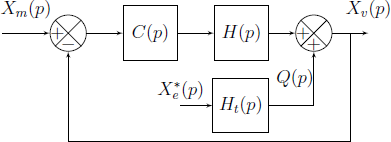
\includegraphics[width=\linewidth]{fig_03}
%%\end{center}
%
%L’équation du mouvement de l’équipage mobile est donnée par : 
%$$
%m\ddot{L}(t)=-rL(t)+\left(S_a-S_b \right)p_e(t)-f'\dot{L}(t).
%$$
%
%\subparagraph{}
%\textit{En déduire, en tenant compte de l’équation du débit, deux équations liant $L(p)$, $P_e(p)$ et $Q_e(p)$, transformées de Laplace de $L(t)$, $P_e(t)$ et $Q_e(t)$. }
%
%Les conditions initiales sont supposées nulles.
%
%\subparagraph{}
%\textit{Sur le document réponse, compléter le schéma bloc de l’ensemble (sans le distributeur hydraulique), l’entrée étant la pression d’huile régulée $P_r(p)$ et la sortie la pression d’épreuve dans le tube $P_e(p)$.}
%
%
%
%La figure suivante représente la réponse de l’ensemble de mise sous pression pour un échelon de 250 bars : $P_r$ est la pression d’huile en sortie du régulateur, $P_h$ la pression d’huile dans le distributeur et $P_e$ la pression d’eau dans le tube.
%
%\begin{center}
%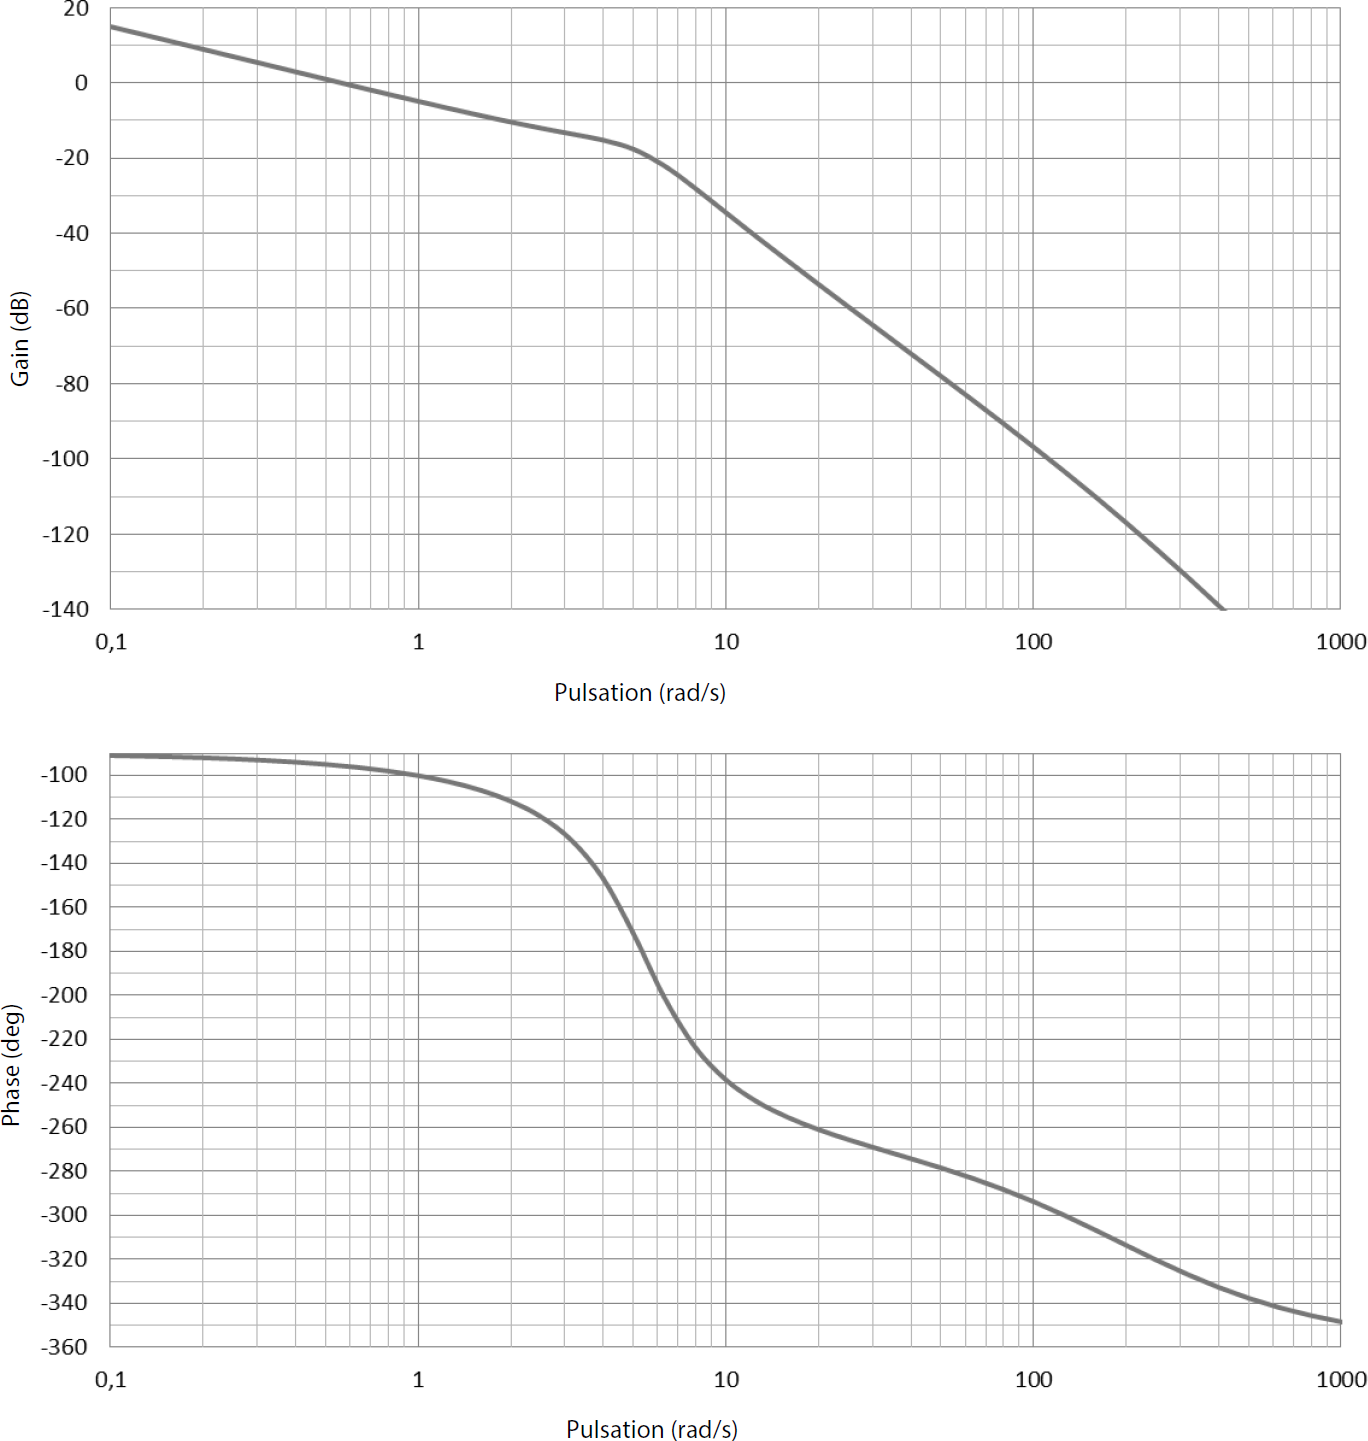
\includegraphics[width=\linewidth]{fig_04}
%\end{center}
%
%\subparagraph{}
%\textit{À partir de ces réponses temporelles, proposer une expression numérique des fonctions de transfert $P_h(p)/P_r(p)$, $P_e(p)/P_r(p)$. Justifier vos valeurs numériques.}
%
%\vspace{.25cm}
%
%De nombreuses fuites au niveau de l’outillage avant influent sur la réponse. À cause de ces fuites, le débit d’eau en entrée du tube est $Q’_e(t) = Q_e(t)-\Delta Q_e$, $\Delta Q_e$ étant le débit de fuite, supposé constant.
%La suivante représente la réponse de l’ensemble de mise sous pression à un échelon de 250 bars avec fuite d’eau à partir de \SI{35}{s}. Le débit de fuite est supposé pour cette étude, égal à $\Delta Q_e = \SI{2}{10^{-3}.m^3/s}$.
%
%\begin{center}
%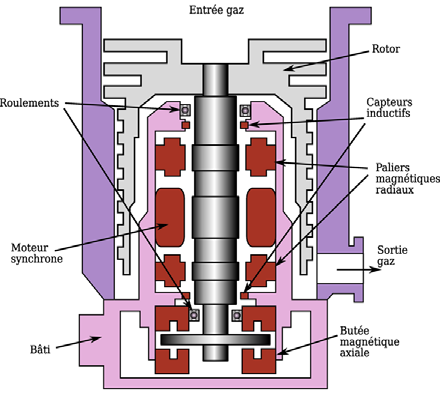
\includegraphics[width=\linewidth]{fig_05}
%\end{center}
%
%\subparagraph{}
%\textit{À partir de ces réponses temporelles, proposer une expression numérique de la fonction de transfert en régulation $\dfrac{P_e(p)}{\Delta Q_e(p)}$.}
\fi

\subsection*{Mise en place d'un asservissement de pression.}
\ifprof
\else
Pour limiter l’erreur statique due aux fuites, on envisage d’asservir la pression d’eau dans le tube. L’objectif est ici de proposer un réglage du correcteur pour répondre aux critères du cahier des charges.
La pression d’eau à l’intérieur du tube est mesurée par un capteur de pression. Le schéma-blocs de l’asservissement est défini ci-dessous.

\begin{center}
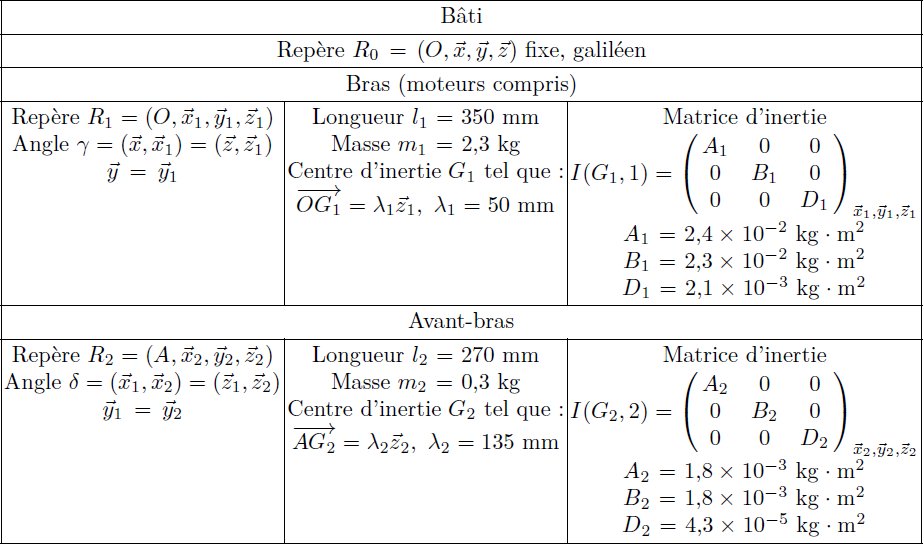
\includegraphics[width=\linewidth]{fig_06}
\end{center}

\begin{itemize}
\item $P_{\text{con}}(p)$ 	: 	pression de consigne d’eau dans le tube (Pa);
\item $P_e(p)$ 	:	pression d’eau dans le tube (Pa);
\item $U_c(p)$ 	: 	tension de commande du régulateur de pression (V);
\item $P_r(p)$ 	:	pression d’huile régulée (Pa);
\item $\Delta Q_e(p)$ 	:	débit de fuite ($\text{m}^3/\text{s}$);
\item $U_m(p)$ 	:	tension de mesure du capteur (V).
\end{itemize}

Hypothèses : 
\begin{itemize}
\item quels que soient les résultats précédents, l’ensemble de mise sous pression \{tube + distributeur + multiplicateur de pression\} est défini par les transmittances suivantes :
$H_{\text{pre}} (p)=\dfrac{K_m}{1+T_1 p}$ et $H_{\text{fui}} (p)=\dfrac{K_f}{1+T_1 p}$
avec $K_m = 3,24$; $K_f = \SI{2,55}{10^{10} Pa/(m^3/s)}$; $T_1  =\SI{10}{s}$; 
\item l’ensemble \{pompe+régulateur de pression\} est modélisé par la fonction de transfert :
$H_{\text{pom}} (p)=\dfrac{K_{\text{pom}}}{1+T_2 p}$ avec $K_{\text{pom}} = \SI{1,234}{10^7 Pa/V}$; 	$T_2 = \SI{5}{s}$;
\item le capteur est modélisé par un gain pur :	$K_{\text{cap}}= \SI{2,5}{10^{-8}.V/Pa}$.
\end{itemize}

La pression de consigne est de $P_{\text{con}} = \SI{800}{bars}$ et les débits de fuite sont estimés à $\Delta Q_e = \SI{5}{10^{-4} m^3/s}$.

On rappelle que le cahier des charges concernant le réglage de la pression de test est le suivant :
\begin{center}
\begin{tabular}{|l|p{5cm}|}
\hline
Stabilité : & marge de phase de $60\degres$

 marge de gain de \SI{12}{dB} \\ \hline
Rapidité :	&temps d’établissement $t_e < \SI{40}{s}$ \\ \hline
Précision :&	erreur statique < 5\% soit pour une consigne de 800 bars :

erreur statique due à la consigne : $\varepsilon_{\text{con}} < 5\%$ 

erreur statique due à la perturbation $\varepsilon_{\text{pert}} < \SI{40}{bars}$ \\ \hline

Amortissement :&	pas de dépassement \\ \hline
\end{tabular}
\end{center}

Dans le cas d’un système bouclé convenablement amorti, on pourra utiliser, sans aucune justification, la relation : 	$t_e \omega_{\SI{0}{dB}}=3$ 
où $\omega_{\SI{0}{dB}}$ désigne la pulsation de coupure à \SI{0}{dB} en boucle ouverte et $t_e$ le temps d’établissement en boucle fermée vis-à-vis d’un échelon de consigne :
\begin{itemize}
\item $t_e = t_m$, temps du 1\ier maximum si le dépassement est supérieur à 5\%;
\item $t_e = t_R$, temps de réponse à 5\% si le dépassement est nul ou inférieur à 5\%.
\end{itemize}
\fi

\subsection*{Correction proportionnelle}
On envisage tout d’abord un correcteur de type proportionnel : $C(p)=K_p$. 



\subparagraph{}
\textit{Transformer le schéma-blocs pour se ramener à un système à retour unitaire.}
\ifprof
\begin{corrige}~\\

\begin{center}
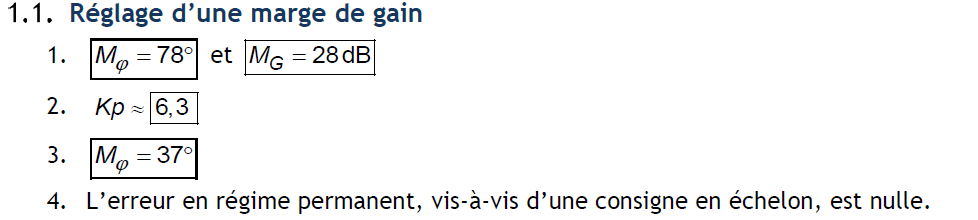
\includegraphics[width=\linewidth]{cor_01}
\end{center}
\end{corrige}
\else
\fi

\subparagraph{}
\textit{Déterminer, en fonction de $K_p$ , $\varepsilon_{\text{con}}$ définie comme l’erreur statique pour une entrée consigne $P_{\text{con}}$ de type échelon, dans le cas où le débit de fuite est nul.}
\ifprof
\begin{corrige}
Dans ce cas, le système est de classe 0. L'erreur statique est donc de $\varepsilon_{\text{con}}=\dfrac{P_{\text{con}}}{1+K_{\text{cap}}K_pK_mK_{\text{pom}}}$.
\end{corrige}
\else
\fi

\subparagraph{}
\textit{Proposer un réglage de $K_p$ pour limiter $\varepsilon_{\text{con}}$ à la valeur spécifiée dans le  cahier des charges.}
\ifprof
\begin{corrige}

Pour que l'erreur soit inférieure à 5\% : 

$\dfrac{P_{\text{con}}}{1+K_{\text{cap}}K_pK_mK_{\text{pom}}}<0,05 P_{\text{con}}$

$\Leftrightarrow 1<0,05 \left(1+K_{\text{cap}}K_pK_mK_{\text{pom}}\right)$

$\Leftrightarrow \dfrac{0,95}{0,05K_{\text{cap}}K_mK_{\text{pom}}}<K_p$.
On a donc $K_p>19$.
\end{corrige} 
\else
\fi

\subparagraph{}
\textit{Dans le cas où la consigne de pression est nulle,  déterminer en fonction de $K_p$  $\varepsilon_{\text{pert}}$ définie comme l’erreur statique pour une perturbation $\Delta Q_e$ de type échelon, dans le cas où la consigne de pression est nulle.}
\ifprof
\begin{corrige}
Dans ce cas, on a toujours un système dont la BO est de classe 1 et : 
$\varepsilon_{\text{pert}}=\dfrac{\Delta Q_e K_f}{1+K_{\text{cap}}K_pK_mK_{\text{pom}}}$.

\end{corrige}
\else
\fi

\subparagraph{}
\textit{Proposer un réglage de $K_p$ pour limiter $\varepsilon_{\text{pert}}$ à la valeur spécifiée au cahier des charges.}
\ifprof
\begin{corrige}
Pour $\Delta Q_e = \SI{5}{10^{-4} m^3/s}$ on souhaite $\varepsilon_{\text{pert}} < \SI{40}{bars}$. En conséquence, 
$\dfrac{\Delta Q_e K_f}{1+K_{\text{cap}}K_pK_mK_{\text{pom}}} <40$ 
$\Leftrightarrow  \dfrac{\Delta Q_e K_f -40}{40K_{\text{cap}}K_mK_{\text{pom}}}<K_p$. On a donc $K_p>2,19$.
\end{corrige}
\else
\fi

\subparagraph{}
\textit{Proposer un réglage de $K_p$ pour vérifier le critère d’amortissement.}
\ifprof
\begin{corrige}
Pour avoir aucun dépassement, il est nécessaire que, si la FTBF du système est d'ordre 2, on ait $\xi\geq 1$. (Si la FTBF est d'ordre 1, il n'y aura pas de dépassement, si la FTBF est d'ordre supérieur à 2 il n'y a pas de résultat connu.)

On a donc, avec un débit de fuite nul, $\dfrac{P_e(p)}{P_{con}(p)}
=\dfrac{K_{\text{cap}}K_p\dfrac{K_{\text{pom}}}{1+T_2 p}\dfrac{K_{m}}{1+T_1 p}}{1+K_{\text{cap}}K_p\dfrac{K_{\text{pom}}}{1+T_2 p}\dfrac{K_{m}}{1+T_1 p}}$

$=\dfrac{K_{\text{cap}}K_pK_{\text{pom}} K_{m}}{\left(1+T_1 p\right)\left(1+T_2 p\right)+K_{\text{cap}}K_pK_{\text{pom}} K_{m}}$

%$=\dfrac{
%K_{\text{cap}}K_pK_{\text{pom}} K_{m}
%}{
%\left(1+T_1 p\right)\left(1+T_2 p\right)+K_{\text{cap}}K_pK_{\text{pom}} K_{m}
%}$

$=\dfrac{
K_{\text{cap}}K_pK_{\text{pom}} K_{m}
}{
\left(T_1 +  T_2\right) p + T_1T_2 p^2+1+K_{\text{cap}}K_pK_{\text{pom}} K_{m}
}$.

On a alors : $\omega_0 = \sqrt{\dfrac{1+K_{\text{cap}}K_pK_{\text{pom}} K_{m}}{T_1T_2}}$
et

$\xi=\dfrac{1}{2}\dfrac{T_1+T_2}{\sqrt{T_1T_2 \left(1+K_{\text{cap}}K_pK_{\text{pom}} K_{m}\right)}}$.
 
En conséquence, $\xi>1\Leftrightarrow \dfrac{\left(T_1+T_2\right)^2-4T_1T_2 }{4T_1T_2 K_{\text{cap}}K_{\text{pom}} K_{m}} > K_p $ et donc $K_p<0,125 $.

\end{corrige}
\else
\fi


\subparagraph{}
\textit{À partir des résultats des questions précédentes, conclure quant au choix d’un correcteur proportionnel.}
\ifprof
\begin{corrige}
On a donc : 
\begin{itemize}
\item $K_p>19$;
\item $K_p> 2,19$;
\item $K_p<0,125 $.
\end{itemize}
Les 3 conditions sont incompatibles. Un autre correcteur doit être envisagé.
\end{corrige}

\else
\fi

\subsection*{Correction proportionnelle intégrale}
On se propose de corriger le système avec le correcteur défini sur le schéma-blocs ci-dessous :
\begin{center}
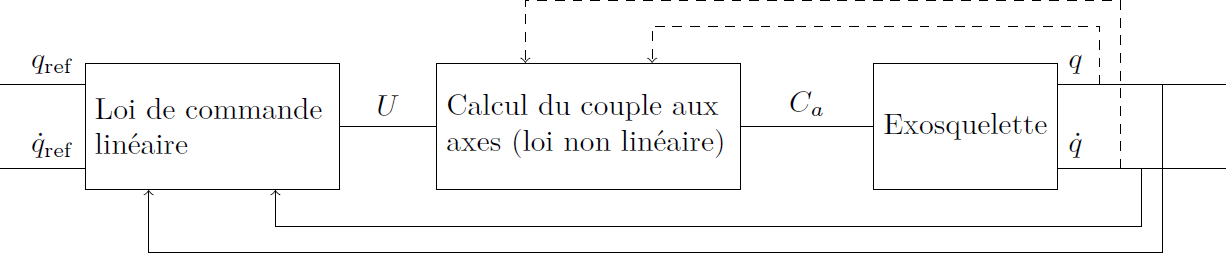
\includegraphics[width=.4\linewidth]{fig_07}
\end{center}


\subparagraph{}
\textit{Déterminer la fonction de transfert $C(p)$ de ce correcteur.}
\ifprof
\begin{corrige}
On a $C(p)=\dfrac{K_i}{p}+K_p = \dfrac{K_i+K_p p}{p}= \dfrac{K_i}{p}\left(1+\dfrac{K_p}{K_i} p\right)$.
\end{corrige}
\else
\fi



\subparagraph{}
\textit{Tracer l’allure de son diagramme de Bode en fonction des coefficients $K_i$ et $K_p$.}
\ifprof
\begin{corrige}

\end{corrige}
\else
\fi

\subparagraph{}
\textit{Quelle est l’influence d’un tel correcteur sur la précision et la stabilité ? Justifier.}
\ifprof
\begin{corrige}
L'intégrateur va permettre d'annuler l'erreur (du à la consigne et à la perturbation).
De plus, suivant le positionnement du correcteur, le déphasage de -90\degres présent en basse fréquence peut déstabiliser le système.
\end{corrige}
\else
\fi

\subparagraph{}
\textit{Quelle valeur faut-il donner à $\omega_{\SI{0}{dB}}$ pour répondre au critère de rapidité du cahier des charges ?}
\ifprof
\begin{corrige}
On souhaite que $t_e<\SI{40}{s} \Leftrightarrow \dfrac{3}{\omega_{\SI{0}{dB}}}<40 \Leftrightarrow \dfrac{3}{40}<\omega_{\SI{0}{dB}}$ et donc $\omega_{\SI{0}{dB}}>\SI{0,075}{rad.s^{-1}}$.
\end{corrige}
\else
\fi

\subparagraph{}
\textit{Déterminer alors le rapport $T=K_p/K_i$ pour obtenir la marge de phase spécifiée dans le cahier des charges.} 
\ifprof
\begin{corrige}
On désire une marge de phase de 60\degres. Il faut donc que $\varphi\left( \omega_{\SI{0}{dB}}\right)=-120\degres$.
On a $FTBO(p)=\dfrac{K_i}{p}\left(1+\dfrac{K_p}{K_i} p\right)K_{\text{cap}}\dfrac{K_m}{1+T_1p}\dfrac{K_{\text{pom}}}{1+T_2p}$. Et donc :
$\varphi(\omega)=-90+\arctan\left( \dfrac{K_p}{K_i}\omega \right)-\arctan\left( T_1\omega \right)-\arctan\left( T_2\omega \right)$ en $\omega_{\SI{0}{dB}}$ on a : $\varphi(0,075)=-90+\arctan\left( \dfrac{K_p}{K_i}0,075\right)-57=-147+\arctan\left( \dfrac{K_p}{K_i}0,075\right)$. On cherche donc $\dfrac{K_p}{K_i}$ tel que $-147+\arctan\left( \dfrac{K_p}{K_i}0,075\right)=-120 \Rightarrow \arctan\left( \dfrac{K_p}{K_i}0,075\right)=27\Rightarrow \dfrac{K_p}{K_i}0,075 = 0,51 \Rightarrow \dfrac{K_p}{K_i}= 6,79$. Ainsi pour avoir une marge de phase supérieure à 60\degres, on doit avoir $T=\dfrac{K_p}{K_i}> 6,79$.
\end{corrige}
\else
\fi

%0,8911

\subparagraph{}
\textit{En déduire les valeurs de $K_p$ et de $K_i$ qui permettent de régler rapidité et marge de phase.}
\ifprof
\begin{corrige}
On souhaite que le gain soit nul lorsque $\omega_{\SI{0}{dB}}=\SI{0,075}{rad.s^{-1}}$. 

On a $G_{\text{dB}}(\omega)=20\log\left(\sqrt{1+\dfrac{K_p^2}{K_i^2}\omega^2} \right) + 20\log K_i +20\log\left( K_{\text{cap}}K_{\text{pom}}K_m\right)-20\log\omega +20\log\left(\sqrt{1+\dfrac{K_p^2}{K_i^2}\omega^2} \right)
-20\log\left(\sqrt{1+T_1^2\omega^2} \right)
-20\log\left(\sqrt{1+T_2^2\omega^2} \right)$. 

$G_{\text{dB}}\left(\omega_{\SI{0}{dB}}\right) =0 \Rightarrow K_i = 0,089$ et $K_p=0,615$.


%$20\log\left(\sqrt{1+\dfrac{K_p^2}{K_i^2}\omega^2} \right) + 20\log K_i -19,99=20\log\left(\sqrt{K_i^2+K_p^2\omega^2} \right) -19,99$.
%On a alors 
%$20\log\left(K_i\sqrt{1+T^2\omega^2} \right) -19,99=0 \Rightarrow K_i =\dfrac{10^{\dfrac{19,99}{20}}}{\sqrt{1+T^2\omega^2} }$
%et $K_i = 0,76$. 
\end{corrige}
\else
\fi

\subsection*{Bilan}

On donne les diagrammes de Bode en gain et en phase de la fonction de transfert en boucle ouverte corrigée avec le correcteur Proportionnel Intégral déterminé précédemment.

\begin{center}
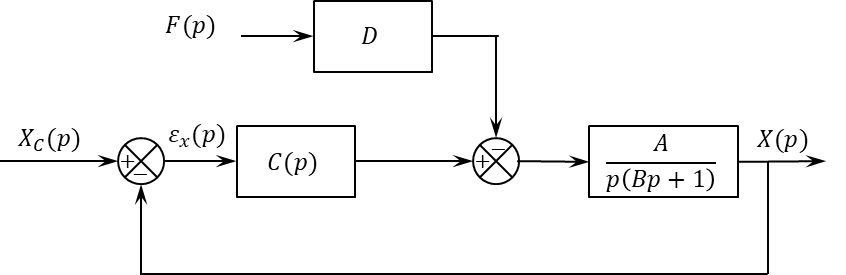
\includegraphics[width=\linewidth]{fig_08}
\end{center}


On donne ensuite sa réponse temporelle avec et sans débit de fuite pour une pression de consigne d’eau de \SI{800}{bars}.


\begin{center}
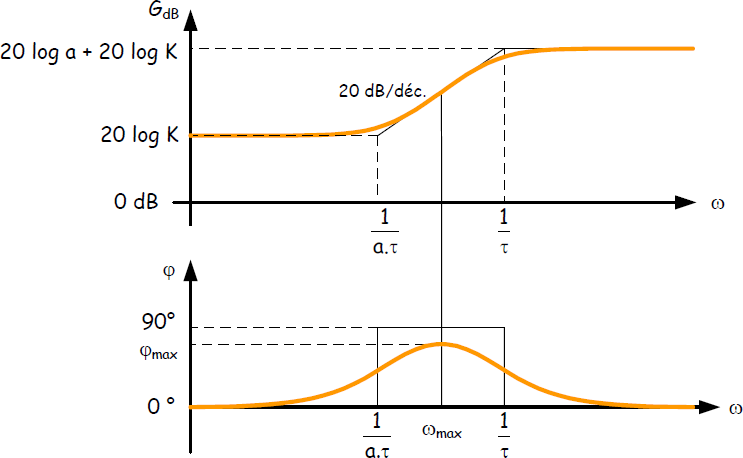
\includegraphics[width=\linewidth]{fig_09}
\end{center}

\subparagraph{}
\textit{La réponse du système est-elle satisfaisante au regard du cahier des charges ? Justifier.}
\ifprof
\begin{corrige}

\end{corrige}
\else
\fi



\end{multicols}

%\end{document}
%\newpage
%
%\subparagraph{}\textit{}
%\begin{center}
%\includegraphics[width=\linewidth]{}
%%\textit{}
%\end{center}
%
%
%%\newpage
%
%%\begin{center}
%%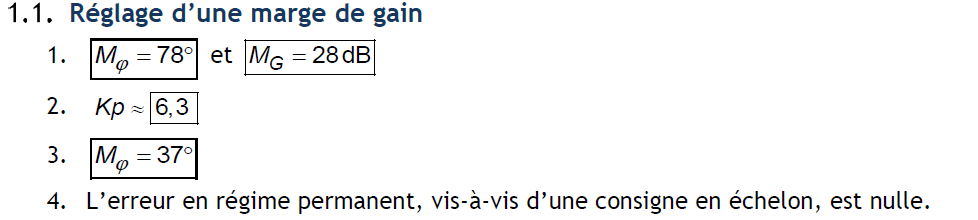
\includegraphics[width=\linewidth]{cor_01}
%%\textit{}
%%\end{center}
%
%
%
%
%
%
%\begin{center}
%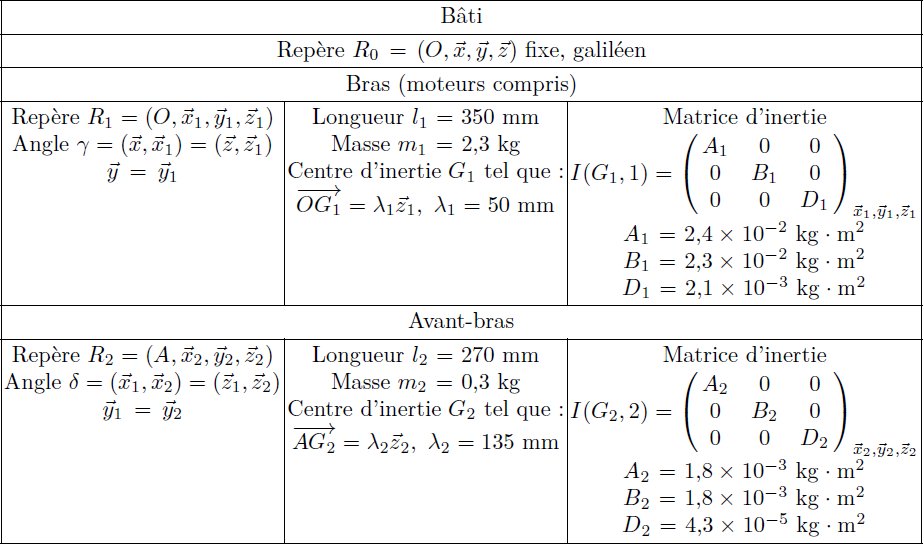
\includegraphics[width=\linewidth]{fig_06}
%%\textit{}
%\end{center}
%\begin{center}
%\includegraphics[width=\linewidth]{img_04}
%%\textit{}
%\end{center}
%
